In this chapter, we'll begin

\todo{introduction}

\section{Intersection Theory}

Throughout this chapter, we'll adopt the convention that $X$ is an ambient $n$-dimensional oriented manifold with boundary, and $M$ and $N$ are closed manifolds. We'll assume that all closed submanifolds of $X$ and smooth maps from a closed manifold to $X$ avoid the boundary.

\begin{definition}\label{def:transverse-intersection-basic}
	Two submanifolds $M,N\subset X$ are said to \defn{intersect tranversally} or to be \defn{transverse} if for all points $p\in M\cap N$ we have $\T_p M\oplus \T_p N = \T_p X$.
\end{definition}

\begin{figure}[ht]
	\centering
	\import{graphics/temp-diagrams/}{transverse-intersection.pdf_tex}
	\medskip
	\caption{Examples and non-examples of transverse intersections in $\R^3$.}\label{fig:transverse-intersection}
\end{figure}

If we lose the assumption that the spaces we're considering aren't smoothly embedded submanifolds of the ambient space, but rather images of a smooth map then this definition can be slightly generalized.

\begin{definition}\label{def:transverse-intersection}
	If $f : N \to X$ and $g : M \to X$ are smooth maps, we say that $f$ and $g$ are \defn{transverse} if for all $p\in N$ and $q\in M$ with $f(p)=g(q)=x\in X$, we have
	\[
		\T_x X = df_p(\T_p N) \oplus dg_q(\T_q M).
	\]
\end{definition}

\begin{remark}
	When $f$ and $g$ are embeddings, this recovers \cref{def:transverse-intersection-basic}.
\end{remark}

While it's easy to come up with examples of manifolds which aren't transverse, there is a mathematical sense in which ``almost all'' submanifolds intersect transversally.

\begin{theorem}
	Let $C^\infty(N,X)$ be the space of all maps from a compact manifold $N$ to some ambient manifold $X$. If we fix a submanifold $M\subset X$, then the subset
	\[
		C^\infty_{\mathrm{tv.}\,M}(N,X)=\{ f : N \to X  f\textrm{ is transverse to } M\}\subset C^\infty(N,X)
	\]
	of maps transverse to $M$ is a dense subset of $C^\infty(N,X)$.
\end{theorem}

\begin{proof}
	See the proof of Theorems~6.35 in \cite{lee2012smooth}.
\end{proof}

In simpler terms, this density of transverse maps implies that transversality is a \defn{stable}[stable property] and \defn{generic}[generic property] property. Stability in this context means that it is resilient to perturbations (if a map is transverse to $M$, perturbing it slightly will keep it transverse to $M$), and generality means that if a map is not transverse to $M$, we can perturb it slightly to make it transverse.
What this means for us is that without much loss of generality, we can assume that all manifolds and smooth maps intersect transversally.

\begin{figure}[ht]
	\centering
	\import{graphics/temp-diagrams/}{perturbing-intersection-transverse.pdf_tex}
	\medskip
	\caption{Perturbing a manifold embedding to get a transverse intersection.}\label{fig:perturbing-intersections-transverse}
\end{figure}

The observant reader might remark that there isn't a way of measuring distances between maps in $C^\infty(N,X)$, this would require more than just the topological data we have access to. We do however have a notion of homotopy, so whenever refer to stability, generality, and perturbation, we use the following formal definition.

\begin{definition}
	Suppose we have a property $\mathcal{P}$ of functions between topological spaces.
	\begin{enumerate}
		\item The property $\mathcal{P}$ is said to be \defn{stable}[stable property] if for every function $f : X \to Y$ satisfying $\mathcal{P}$ and homotopy $H : X\times[0,1]\to Y$ with $H(x,0) = f(x)$, there exists an $\varepsilon>0$ such that for all $s\in [0,\varepsilon)$, the function $H(x,s)$ also satisfies $\mathcal{P}$.
		\item The property $\mathcal{P}$ is said to be \defn{generic}[generic property] if for every function $f : X \to Y$ \emph{not} satisfying $\mathcal{P}$ and arbitrary $\varepsilon>0$, there is a homotopy $H : X\times [0,\varepsilon] \to Y$ with $H(x,0)=f(x)$ such that the function $H(x,\varepsilon)$ satisfies $\mathcal{P}$.
	\end{enumerate}
\end{definition}

\subsection{The Oriented Intersection Number}

One of the fundamental properties concerning transverse maps is that they behave well when taking intersections, or more generally when taking preimages. This forms the backbone of the intersection theory of manifolds.

\begin{theorem}[Preimage Theorem]\label{thm:preimage}
	If $f : N \to X$ is a smooth map transverse to a submanifold $M\subset X$ then $S=f^{-1}(M)\subset N$ is a submanifold with the same codimension in $N$ as $M$ in $X$.
\end{theorem}
\begin{proof}
	See the proof of Theorem~6.30 in \cite{lee2012smooth}.
\end{proof}

\begin{remark}\label{rmk:symmetric-preimage-theorem}
	We can get a symmetric version of this theorem as a straightforward corollary. If we have two transverse maps $f : N\to X$ and $g : M\to X$, then the map $f\times g : N\times M \to X\times X$ is transverse to the diagonal submanifold $\Delta\subset X\times X$. \cref{thm:preimage} will then imply that
	\[
		(f\times g)^{-1}(\Delta) \subset M\times N
	\]
	is a submanifold. When $g$ is an embedding, $(f\times g)^{-1}(\Delta)$ can be projected down onto $M$ to get the preimage $f^{-1}(M)$.
\end{remark}

If the manifolds involved in \cref{thm:preimage} are orientable, this preimage $S$ admits a canonical orientation by the following procedure. First of all, recall that for any embedded manifold $M\subset X$ there is an exact sequence of vector bundles by quotienting
\begin{equation}\label{eq:oriented-intersection-number-1}
	\begin{tikzcd}
		0 & {\T M} & {\T X} & {\T X/M} & 0
		\arrow[from=1-1, to=1-2]
		\arrow[from=1-2, to=1-3]
		\arrow[from=1-3, to=1-4]
		\arrow[from=1-4, to=1-5]
	\end{tikzcd}
\end{equation}
where $\T X/M$ is the normal bundle of $M\subset X$. Using the orientations of $X$ and $M$, we can use this exact sequence to get an orientation of the normal bundle $\T X/M$. At every point $p\in S$ of the preimage, the differential map $df$ connects the sequence \cref{eq:oriented-intersection-number-1} to the normal bundle sequence for the embedding $S\subset N$.
\begin{equation}\label{eq:oriented-intersection-number-2}
	\begin{tikzcd}
		0 & {\T_pS} & {\T_p N} & {\T_p N/S} & 0 \\
		0 & {\T_{f(p)}M} & {\T_{f(p)}X} & {\T_{f(p)}X/M} & 0
		\arrow[from=1-1, to=1-2]
		\arrow[from=1-2, to=1-3]
		\arrow["{df_p}", from=1-2, to=2-2]
		\arrow[from=1-3, to=1-4]
		\arrow["{df_p}", from=1-3, to=2-3]
		\arrow[from=1-4, to=1-5]
		\arrow["{df_p}", from=1-4, to=2-4]
		\arrow[from=2-1, to=2-2]
		\arrow[from=2-2, to=2-3]
		\arrow[from=2-3, to=2-4]
		\arrow[from=2-4, to=2-5]
	\end{tikzcd}
\end{equation}
In this diagram \cref{eq:oriented-intersection-number-2}, the rightmost vertical map is an isomorphism by the transversality of $f$ and $M$. This means that we can pullback the orientation on $\T_{f(p)} X/M$ to $\T_p N/S$. Since $\T_p N$ is oriented, the usual ``2-out-of-3'' rule applied to the top row of \cref{eq:oriented-intersection-number-2} gives an orientation of $\T_p S$. See \cref{fig:preimage-orientation} for an example of this orienting procedure.

\begin{figure}[ht]
	\centering
	\import{graphics/temp-diagrams/}{preimage-orientation.pdf_tex}
	\medskip
	\caption{Orienting a preimage (assuming a clockwise orientation on $X$ and $N$).}\label{fig:preimage-orientation}
\end{figure}

When $M$ and $N$ have complementary dimensions, the preimage $S=f^{-1}(N)\subset M$ is a compact oriented $0$-dimensional manifold. For each point $p\in S$, we have $\T_p S=0$ so the map $\T_p N\to \T_p N/S$ in \cref{eq:oriented-intersection-number-2} is an isomorphism. The orientation of $N$ gives an orientation of $\T_p N$, and the preimage orientation procedure gives us an orientation of $\T_p N/S$. Now we can define:

\begin{definition}
	The \defn{local (oriented) intersection number}[oriented intersection number (local)] of $f$ and $M$ at $p\in S$ is
	\[
		\#_p^X(f, M) = \begin{cases}
			+1 & \T_p N/S \textrm{ has the same orientation as } \T_p N,     \\
			-1 & \T_p N/S \textrm{ has the opposite orientation to } \T_p N.
		\end{cases}
	\]
\end{definition}
Summing over all of the local intersection numbers gives a global quantity.
\begin{definition}
	The \defn{(oriented) intersection number}[oriented intersection number] of a smooth map $f : N \to X$ intersecting a submanifold $M\subset X$ transversally is
	\[
		\#^X(f, M) = \sum_{p\in S} \#_p^X(f, M) \in \Z.
	\]
\end{definition}

\begin{remark}\label{rmk:symmetric-intersection-number}
	For a more symmetric version of this definition when two smooth maps $f : N \to X$ and $g : M \to X$ intersect transversally, we could take inspiration from \cref{rmk:symmetric-preimage-theorem} and define the oriented intersection number of the smooth maps $f$ and $g$ as
	\[
		\#^X(f,g) = \#^{X\times X}(f\times g, \Delta).
	\]
	This symmetric intersection number is graded commutative in the dimensions of $M$ and $N$, i.e.
	\begin{equation}\label{eq:intersection-number-graded-commutative}
		\#^X(f,g) = (-1)^{\dim M\cdot \dim N} \#^X(g,f)
	\end{equation}
\end{remark}

Just as the property of transversality is stable -- resilient to homotopic perturbations -- so too is the oriented intersection number. This follows as a corollary to a more general theorem.

\begin{theorem}
	If $W$ is a compact oriented manifold with boundary, and $H : W \to X$ is a smooth map, then $\#^X(\partial H, M)=0$. Here, we use the notation $\partial H : \partial W \to X$ to refer to the restriction of $H$ to the boundary of $W$.
\end{theorem}

\begin{corollary}
	If $H : [0,1]\times N \to X$ is a smooth homotopy, then $\#^X(H_0, M) = \#^X(H_1, M)$.
\end{corollary}

Applying the construction of the symmetric oriented intersection number gives a map
\begin{equation}\label{eq:oriented-intersection-number-homotopy}
	\lkxfunc{\#^X}{[N,X]\times [M,X]}{\Z}{f,g}{\#^X(f,g)}
\end{equation}
This is a geometric precursor to the intersection form of a manifold, a central object of study in geometric topology.

\begin{remark}
	If we don't assume orientations, we can still get a homotopy invariant intersection number, however we must reduce mod $2$. In this case, we could simply define 
	\[
		\#_2^X(f,M) = |S|\mod 2.
	\]
	This is called the \defn{unoriented intersection number}.
	\todo{elaborate}
\end{remark}

Finally, we'll state a useful result in computer self-intersection numbers -- a way to compute the intersection number of a submanifold with itself.

\begin{theorem}\label{thm:euler-number-self-intersection}
	If $M$ is a closed $m$-dimensional submanifold of a $2m$-dimensional submanifold $X$ then we have
	\[
		\#^X(M, M) = \chi(\T X/M)
	\]
	where $\chi(\T X/M)$ is the Euler number of the normal bundle of $M$.
\end{theorem}
\begin{proof}
	\todo{todo}
\end{proof}

\begin{corollary}\label{thm:euler-number-self-intersection-corollary}
	The Euler number $\chi(\xi)$ of an oriented real vector bundle $\xi : E \to B$ over a compact oriented manifold can be expressed as the intersection number
	\[
		\#^E(z,z) = \chi(\xi)
	\]
	where $z : B \to E$ is the zero section.
\end{corollary}

\todo{add 1.C from \cite{levine1985lectures}}

\subsection{Homology Classes and Submanifolds}

Let $f : N\subset X$ be a smooth map from a compact oriented $p$-dimensional manifold $N$ to $X$. The data of an orientation on a closed manifold gives a fundamental class $[N]\in \H_p(N)$ which can be pushed forward along the map $f : N \hookrightarrow X$ to give us a homology class $f_* [N]\in \H_p(X)$. This is the homology class associated to a smooth map $N\to X$.
This correspondence behaves nicely with respect to perturbations, and thus as we will later see, with transversality.
Suppose $H : N\times [0,1] \to X$ is a homotopy with $H(x,0)=f(x)$ which perturbs the map $f$. For any $\varepsilon>0$, the map $f_\varepsilon : N \to X$ given by $f_\varepsilon(x)=H(x,\varepsilon)$ is homotopic to $f$ and hence induces the same map on homology $\H_p(N)\to \H_p(X)$. The homology class associated to a map $f : N \to X$ thus solely depends on the homotopy type of $f$ so we get a map
\[
	\lkxfunc{}{[N,X]}{\H_p(X).}
\]
Letting $N=S^p$, we can see that this is a generalization of the Hurewicz homomorphism which links homotopy groups to homology groups via a map $\pi_p(X) \to \H_p(X)$.
As with the Hurewicz homomorphism, this correspondence is generally not surjective or injective. If a space is $k$-connected for $k\geq 1$ then we have a Hurewicz isomorphism $\pi_{k+1}(X) \to \H_{k+1}(X)$ which means that every homology cycle in $\H_{k+1}(X)$ can at least be represented by a smooth map of a sphere $S^{k+1}$ into $X$. This smooth map might have ``double-points'', i.e. when multiple points of the sphere map to the same point in the image and prevent the smooth map from being an embedding.

\begin{example}
	In the punctured plane $X=\R^2\setminus \{0\}$ with homology $\H_1(X)\cong \Z$, the only homology cycles which can be represented by embedded submanifolds are $0,\pm 1$, by a circle not containing the origin and circles of both orientations surrounding the origin respectively. A smooth map representing a cycle of higher degree would necessarily have a double-point as in \cref{fig:double-point}.
\end{example}

\begin{figure}[ht]
	\centering
	\import{graphics/temp-diagrams/}{double-point.pdf_tex}
	\caption{A double-point in a smooth map representing $\pm 2\in \H_1(\R^2\setminus\{0\})$.}\label{fig:double-point}
\end{figure}

That being said, many specially constructed manifolds we will consider in this chapter will at least have a basis by embedded submanifolds, and every homology class will admit a representation by a smooth map. For a classical account of some issues that can arise when representing homology classes by smooth maps, see Chapter II of Ren\'e Thom's seminal paper \cite{thom1954}.

\begin{remark}
	In some special cases, homology classes can \emph{always} be represented by embedded submanifolds. For instance, if $X$ is a $4$-manifold, there are isomorphisms
	\[
		\H^2(X; \Z) \cong [X, K(\Z,2)] \cong [X, \CP^\infty] \cong [X,\CP^2],
	\]
	where the first is the representability of singular cohomology by the Eilenberg-Maclane spectrum, the second identifies $\CP^\infty$ as a $K(\Z,2)$ space, and the third uses the cellular approximation theorem. Any cohomology cycle $\omega\in \H^2(X)$ can be represented by a smooth function $f : X \to \CP^2$. If we choose this function to be transverse to $\CP^1\subset \CP^2$, then $f^{-1}(\CP^1)$ is an embedded $2$-dimensional submanifold of $X$ which corresponds to a Poincar\'e dual class to $\omega$. When $X$ is a compact manifold, Poincar\'e duality tells us that all $2$-dimensional homology cycles can be represented by embedded submanifolds in this way. This is one reason why $4$-manifolds (especially simply-connected $4$-manifolds) are such wonderful geometric objects of study!
\end{remark}

Now let's see if our previously defined notion of an oriented intersection number transfers over as an operation on homology classes. Recall that by the Poincar\'e-Lefschetz duality for compact manifolds with boundary, there is an isomorphism
\[
	\lkxfunc{}{\H^{n-p}(X,\partial X)}{\H_p(X)}{\omega}{\omega\frown [X,\partial X]}
\]
given an orientation class $[X,\partial X]\in \H_n(X, \partial X)$. Under this duality, there is a geometric interpretation of the cup product on cohomology cycles as the oriented intersection number for submanifolds representing the dual homology cycles (when such a representation is possible). We can define this homology intersection pairing $\tnsv$ as the top map in the commutative square
\begin{equation}\label{eq:homology-intersection}
	\begin{tikzcd}
		{\H_p(X)\otimes \H_q(X)} & {\H_{n-p-q}(X)} \\
		{\H^{n-p}(X, \partial X)\otimes \H^{n-q}(X,\partial X)} & {\H^{2n-p-q}(X,\partial X)}
		\arrow["\tnsv", from=1-1, to=1-2]
		\arrow[tail reversed, from=1-1, to=2-1]
		\arrow[tail reversed, from=1-2, to=2-2]
		\arrow["\smile", from=2-1, to=2-2]
	\end{tikzcd}
\end{equation}
where the vertical maps are the Poincar\'e-Lefschetz isomorphism. Finally, we have our link between the algebra of (co)homology and the differential topology of intersections.

\begin{theorem}
	Suppose $M,N\subset X$ are transverse oriented submanifolds. Then we have
	\[\iota_*[M]\tnsv \iota_*[N] = \#_X(M,N)\]
\end{theorem}
\begin{proof}
	\todo{todo}
\end{proof}

As suggested by the map in \cref{eq:oriented-intersection-number-homotopy}, we now have an entirely algebraic object which encapsulates the geometry of intersections on a manifold.

\begin{definition}
	Let $X$ be an oriented $2m$-dimensional manifold, possibly with boundary. The \defn{intersection form} on middle dimensional homology is the bilinear form
	\[
		\lkxfunc{Q_X}{\H_m(X)_{\mathrm{free}}\otimes \H_m(X)_{\mathrm{free}}}{\Z}{\alpha\otimes \beta}{\alpha\tnsv \beta}
	\]
	where we identify $\H_0(X)\cong \Z$ and $\H_m(X)_{\mathrm{free}}$ denotes the free component of $\H_m(X)$ -- i.e. the quotient by torsion elements.
\end{definition}

\begin{remark}
	There is also an unoriented intersection form which can be defined for unoriented $2m$-manifolds on $\H_m(X;\Z/2)$ by reducing $\alpha\tnsv \beta\mod 2$. This encodes the data of the unoriented intersection number.
\end{remark}

Since $\smile$ is graded-commutative, by \cref{eq:homology-intersection} so is $\tnsv$. Of course, we would expect the graded-commutativity as a generalization of \cref{eq:intersection-number-graded-commutative}. This implies:
\begin{proposition}
	If $m$ is even then $Q_X$ is a symmetric bilinear form and if $m$ is odd then $Q_X$ is a skew-symmetric bilinear form.
\end{proposition}

\begin{convention*}
Moving forward, we'll say that $Q_X$ is \defn{$\bm{m}$-symmetric} to meansymmetric if $m$ is even and skew-symmetric if $m$ is odd.
\end{convention*}

We will see many examples of manifolds and their intersection forms throughout this chapter, so for now let's just consider the most basic non-trivial examples -- complex projective spaces and tori.

\begin{example}\label{exam:intersection-form-complex-projective-space}
	The intersection form for any even (complex) dimensional complex projective plane $\CP^{2m}$ is given by $Q_{\CP^{2m}}=(1)$.  For a geometric view of why this is, let's begin with the vector space $\C^{2m+1}$ with a basis $\{e_0, e_1,\ldots, e_{2m}\}$. Consider the linear subspaces
	\[
		W = \span\{e_0, e_1,\ldots, e_m\}\quad\textrm{and}\quad U = \span\{e_0, e_{m+1},\ldots, e_{2m}\}
	\]
	inside $\C^{2m+1}$. It's clear that their intersection $W\cap U = \span\{e_0\}$ is a complex line. Now, we can pass to the projectivization $\P(\C^{2m+1})=\CP^{2m}$ and realize $W$ and $U$ as embedded submanifolds $\P(W)=\CP^m\subset \CP^{2m}$ and $\P(U)=\CP^m\subset \CP^{2m}$. Since $W$ and $U$ intersected at a line, it's clear that their projectivizations $\P(W)$ and $\P(U)$ intersect at a point. Furthermore, the intersection is transverse and we choose compatible orientations so that it has local intersection number $+1$. Since $\P(W)$ and $\P(U)$ represent the same generating homology class in $\H_{2m}(\CP^{2m})$, it follows that the intersection form is $(1)$.

	\begin{figure}[ht]
		\centering
		\caption{\todo{geometric picture of this in complex projective space}}
	\end{figure}

\end{example}

Note that the intersection form for odd (complex) dimensional complex projective space $Q_{\CP^{2m+1}}=0$ is trivial since odd dimensional complex projective spaces have no middle dimensional homology. We could also reverse the orientation of $\CP^{2m}$ in \cref{exam:intersection-form-complex-projective-space} 

\begin{example}\label{exam:intersection-form-torus}
	The intersection form for a torus $T^{2m}=S^m\times S^m$ can be represented by the matrix
	\[
		Q_{T^{2m}} = \begin{pmatrix}0 & 1 \\ (-1)^m & 0\end{pmatrix}.
	\]
	where we use the basis for $\H_m(T^{2m})$ given by the embedded submanifolds $S^m\times \{p\}$ and $\{p\}\times S^m$ for some $p\in S^m$. If we call these homology classes $\alpha$ and $\beta$, we can normalize orientations so that the local intersection number at their single intersection point $(p,p)$ is $+1$ so that $\alpha\tnsv \beta=1$. It also follows that $\alpha\tnsv \alpha = 0$ since the submanifolds $S^2\times \{p\}$ and $S^2\times \{q\}$ have empty intersection for $p\neq q$ and both represent the homology cycle $\alpha$.
\end{example}

The matrices 
\[
	(1),\quad (-1),\quad H = \begin{pmatrix} 0 & 1 \\ 1 & 0\end{pmatrix},\quad\textrm{and}\quad S=\begin{pmatrix}0 & 1\\ -1 & 0\end{pmatrix}
\]
are the simplest building blocks of bilinear forms over the integers, and correspondingly complex projective spaces and tori are some of simplest building blocks to construct manifolds. We use the notation $H$ because this matrix is sometimes called the \defn{hyperbolic form}, and $S$ because the matrix is referred to as a \defn{symplectic form}. 

\subsection{Connected Sum}

The simplest way to combine two manifolds in order to build a more complicated manifold is the operation of connected sum. 

\begin{definition}
	\todo{definition of connected sum}
\end{definition}

\begin{figure}[ht]
	\centering
	\import{graphics/temp-diagrams/}{connected-sum.pdf_tex}
	\caption{Construction of the connected sum.}\label{fig:connected-sum}
\end{figure}

\begin{proposition}
	\todo{Homology of connected sum}
\end{proposition}

\begin{proposition}\label{prop:connected-sum-intersection-form}
	If $X$ and $Y$ are $2m$-dimensional manifolds, then we have $Q_{X\+Y} = Q_X\oplus Q_Y$.
\end{proposition}
\begin{proof}
	\todo{todo}
\end{proof}

\begin{proposition}\label{prop:reverse-orientation-intersection-form}
	If $X$ is a $2m$-dimensional manifold, then we have $Q_{-X} = -Q_X$ where $-X$ denotes $X$ with reverse orientation.
\end{proposition}
\begin{proof}
	\todo{todo}
\end{proof}

Note that \cref{prop:connected-sum-intersection-form} implies that the intersection form is a homomorphism of commutative monoids, or sets with a commutative associative binary operation and identity elements. On one side, we have the monoid $\mathcal{M}^{2m}$ of oriented compact $2m$-manifolds under the operation of connected sum, and on the other side we have $\mathcal{Q}(\Z)$ of bilinear forms over $\Z$ under the operation of direct sum. We call such bilinear forms \defn{integral bilinear forms}. Similarly, let $\widetilde{\mathcal{M}}^{2m}$ be the monoid of unoriented compact $2m$-manifolds. The maps
\begin{equation}\label{eq:monoid-homomorphism-intersection-form}
	\lkxfunc{}{\mathcal{M}^{2m}}{\mathcal{Q}(\Z)}{X}{Q_X}
	\quad\textrm{and}\quad
	\lkxfunc{}{\widetilde{\mathcal{M}}^{2m}}{\mathcal{Q}(\Z/2)}{X}{Q_X\mod 2}
\end{equation}
are of fundamental importance in surgery theory and in the classification of manifolds, although we will use the former since the manifolds we're interested in are all oriented. For a simple example of classification using intersection forms, let $\mathcal{S}\subset \widetilde{\mathcal{M}}^2$ be the monoid of closed unoriented surfaces under connected sum, then the mod 2 intersection form is actually an isomorphism of commutative monoids
\[
	\lkxfunc{}{\mathcal{S}}{\mathcal{Q}(\Z/2).}
\]

\todo{classification of compact surfaces, presentation of both monoids}
\begin{figure}
	\centering
	\todo{figure}
	\medskip
	\caption{Topology corresponding to the algebraic identity $H\oplus (1)=\oplus^3 (1)$ in $\mathcal{Q}(\Z/2)$.}\label{fig:compact-surfaces-intersection-form-identity}
\end{figure}

This is an example of a model result in algebraic topology -- a complete algebraic classification of a class of manifolds. Better yet, simple algebraic manipulations correspond to non-trivial topological equivalences or modifications. This is part of why intersection forms are so useful -- algebraic intuition scales far better with dimension than geometric intuition does and so bilinear forms are a much more comfortable setting in which to study topology in higher dimensions.

In dimension $4$, we don't get as clean of a result, but it's still remarkable just how much topological information the intersection form is able to capture. Freedman was able to prove in \cite{freedman1982} that the homeomorphism type of a closed simply-connected topological $4$-manifold $X$ is entirely determined by the (oriented) intersection form $Q_X$ and an invariant known as the \defn{Kirby-Siebenmann class} $\kappa(X)\in \H^4(M;\Z/2)$ which vanishes if $X$ admits a PL structure. As a consequence of his classification, it turns out that most bilinear forms over the integers appear as the intersection form of a manifold. 
The algebraic complexities of integral bilinear forms are thus very closely related to topological complexities of manifolds, so studying them as objects in their own right can reveal deep topological insights and useful constructions.
 
The simplest class of manifolds for which the intersection form is an interesting invariant are known as highly-connected manifolds. Highly-connected manifolds contain the minimal amount of (co)homological data for which to define an intersection form, and this makes them an attractive target for classification and construction.
\begin{definition}
	A compact $2m$-dimensional manifold $X$ is said to be \defn{highly-connected} if it is $(m-1)$-connected. By Poincar\'e duality, $X$ has non-trivial (co)homology only in the middle dimension $\H_m(X)$ and in the usual extremal dimensions $\H_0(X)$ and $\H_{2m}(X)$.
\end{definition}

\begin{remark}
	The attempted classification of highly-connected manifolds in dimension $8$ was what led Milnor to the first discovery of an exotic sphere in 1956, see \cite{milnor2000exotic} for an auto-historical account of the discovery.
\end{remark}

\section{Integral Bilinear Forms}\label{sec:integral-bilinear-forms}
Before studying manifolds with a given intersection form in more depth, let's review the general theory of bilinear forms over the integers -- or in other words, understanding the right side of \cref{eq:monoid-homomorphism-intersection-form}. Throughout, let's suppose that $\Lambda$ is a lattice and $Q$ is a bilinear form over $\Lambda$. Recall that under a change of basis matrix $P$, the matrix of the bilinear form transforms as $Q'= P^\intercal QP$. 

\subsection{Invariants}\label{sec:integral-bilinear-forms-invariants}
There are a few basic invariants of bilinear forms which are invariant under this choice of basis.

\begin{definition}[Rank]
	The \defn{rank} of $Q$ is simply the dimension of the lattice $\Lambda$.
\end{definition}

When $Q$ is the intersection form of a manifold, the rank of the intersection form is the middle Betti number $\beta_m = \dim \H_m(X)_{\textrm{free}}$ of the manifold.

\begin{definition}[Signature]
	Write $Q=P^\intercal D P$ for a diagonal real matrix $D$ ($P$ can be a real matrix), then count the number $n^+$ of positive and number $n^-$ of negative eigenvalues, and finally subtract their counts. The resulting difference $n^+ - n^-$ is the \defn{signature}[signature of a bilinear form] of $Q$. Note that zero eigenvalues are ignored. We also sometimes refer to the tuple $(n^+, n^-)$ as the signature of $Q$.
\end{definition}

When $Q$ is the intersection form of a manifold $X$, especially a $4k$-manifold so that the form can have non-zero eigenvalues, the signature of the intersection form is referred to as the \defn{signature}[signature of a manifold] of the manifold, and denoted $\sigma(X)$. This is a topological invariant of fundamental importance, and we will see many of its generalizations and equivalent definitions in \todo{link to other sections}

\begin{remark}
	By Sylvester's Law of Inertia, the rank, signature, and the number of zero eigenvalues completely classifies bilinear forms on a vector space over $\R$ or $\Q$. The case of bilinear forms over $\Z$ is significantly more complex.
\end{remark}

\begin{definition}[Non-Degeneracy]
	A bilinear form is said to be \defn{degenerate}[degenerate bilinear form] if $\det Q=0$ and \defn{non-degenerate}[non-degenerate bilinear form] otherwise.
\end{definition}

\begin{definition}[Unimodularity]
	A bilinear form is said to be \defn{unimodular} if $\det Q=\pm 1$.
\end{definition}

Another way to view a bilinear form is by the homomorphism
\[
	\lkxfunc{Q^\d}{\Lambda}{\Hom(\Lambda, \Z)}{\alpha}{(\beta\mapsto Q(\alpha,\beta)).}
\]
A bilinear form non-degenerate if and only if this map is injective, and unimodular if and only if this map is an isomorphism.

\begin{definition}[Definiteness]
	If for all non-zero elements $\alpha\in \Lambda$ we have $Q(\alpha,\alpha)>0$, then we say that $Q$ is \defn{positive-definite}[positive-definite bilinear form]. On the contrary, if we have $Q(\alpha,\alpha)<0$ for all non-zero elements $\alpha\in \Lambda$, we say that $Q$ is \defn{negative-definite}[negative-definite bilinear form]. Otherwise, $Q$ is said to be \defn{indefinite}[indefinite bilinear form].
\end{definition}

\begin{definition}[Parity]
	If for all elements $\alpha$ we have $Q(\alpha,\alpha)$ even, then $Q$ is said to be \defn{even}[even bilinear form]. Otherwise, we say that $Q$ is \defn{odd}[odd bilinear form].\footnote{Many sources refer to this property as ``type''. Odd forms are then said to be type I and even forms are said to be type II.}
\end{definition}

Examples of integral bilinear forms and manifolds which have them as intersection forms are plentiful. 

\todo{examples thus far, are enough to classify odd indefinite forms}

\todo{skew-symmetric integral bilinear forms}

\subsection{Symmetric Bilinear Forms}

A common source of symmetric bilinear forms over the integers arise from lattices in an inner product space such as Euclidean or Lorentzian space. If $(V,\langle -,-\rangle)$ is an inner product space, a lattice $\Lambda\subset V$ inherits the bilinear form $\langle -,-\rangle$. However, this form is generally not integer valued and so isn't of interest to us. Some very specially constructed lattices however do inherit an integer valued bilinear form.

For instance, in Euclidean space $\R^\ell$ with basis $\{e_1,\ldots, e_\ell\}$ consider the lattice
\[
	\Gamma^\ell = \span\left\{\frac{1}{2}(e_1+\cdots + e_\ell), e_i+e_j \mid i<j\right\}.
\]
When $4\mid \ell$, the Euclidean inner product restricts to an integral bilinear form on this lattice since
\[
	\begin{aligned}
		\left\langle \frac{1}{2}(e_1+\cdots+e_\ell), \frac{1}{2}(e_1+\cdots+e_\ell)\right\rangle &= \frac{\ell}{4},\\
		\left\langle \frac{1}{2}(e_1+\cdots+e_\ell), e_i+e_j\right\rangle &= 1,\\
		\langle e_i+e_j, e_p +e_q\rangle &= \delta_{i,p}+\delta_{i,q}+\delta_{j,p}+\delta_{j,q},
	\end{aligned}
\]
where $\delta$ denotes the Kronecker delta. Since the Euclidean inner product is positive-definite, so is the bilinear form of this lattice. When $8\mid\ell$, the bilinear form of this lattice is even, otherwise it is odd. A special thing happens when $\ell=8$; in this case the lattice becomes unimodular. Geometrically, this means that the fundamental parallelipiped of $\Gamma^8$ has volume $1$. This is rare among lattices, and $\Gamma^8$ is usually called the ${E_8}$ lattice due to its connection to the root system of the exceptional Lie group $\E_8$.

\begin{definition}\label{def:E8-lattice}
	The \defn{$\bm{E_8}$ lattice} or \defn{$\bm{E_8}$ form} is given by the matrix
	\todo{matrix form}
	% \[/
	% 	E_8=
	% 	\begin{pmatrix}
	% 		2 & 1 &   &   &   &   &   &   \\
	% 		1 & 2 & 1 &   &   &   &   &   \\
	% 		  & 1 & 2 & 1 &   &   &   &   \\
	% 		  &   & 1 & 2 & 1 &   &   &   \\
	% 		  &   &   & 1 & 2 & 1 & 0 & 1 \\
	% 		  &   &   &   & 1 & 2 & 1 & 0 \\
	% 		  &   &   &   & 0 & 1 & 2 & 0 \\
	% 		  &   &   &   & 1 & 0 & 0 & 2 \\
	% 	\end{pmatrix}.
	% \]
\end{definition}

\begin{theorem}[Mordell]
	The lattice $E_8=\Gamma^8$ is the only even unimodular positive-definite lattice of rank $8$.
\end{theorem}
\begin{proof}
	\todo{cite}
\end{proof}

In fact, $E_8$ is the smallest even unimodular positive-definite lattice.
\begin{theorem}
	The signature of an even unimodular bilinear form is divisible by $8$.
\end{theorem}
\begin{proof}
	\todo{introduce characteristic elements}
\end{proof}

The attractive properties of the $E_8$ lattice make it a great source of inspiration for topological constructions, however we'd like to emphasize that it does show up naturally in ``the wild''. For instance:

\begin{example}
	In algebraic geometry, the \defn{Kummer K3 surface} defined by the homogeneous polynomial
	\[
		\textrm{K3} = \left\{ [z_0 : z_1 : z_2 : z_3]\in \CP^3 \mid z_0^4 + z_1^4+z_2^4 + z_3^4=0\right\}
	\]
	has the intersection form $Q_{\textrm{K3}} = E_8\oplus E_8 \oplus^3 H$ of signature 16 and rank 22.
\end{example}

While the classification of definite forms is far more complicated, we already have all of the tools to form a complete list of indefinite forms. First, we can prove that:

\begin{theorem}\label{thm:indefinite-bilinear-forms-isomorphic}
	Two unimodular indefinite bilinear forms are isomorphic if they have the same rank, parity, and signature.
\end{theorem}
\begin{proof}
\end{proof}

We are now equipped to list all of the unimodular indefinite forms. 
\begin{proposition}
	Every unimodular indefinite form is isomorphic to either
\[
	\oplus^p (1)\oplus^q (-1)
	\quad\textrm{or}\quad
	\pm \oplus^r E_8 \oplus^{s>0} H.
\]
for some integers $p,q,r,s$. The left side represents all possible odd unimodualr indefinite forms and the right side represents all possible even unimodular indefinite forms.
\end{proposition}
\begin{proof}
	The form $\oplus^p (1)\oplus^q(-1)$ has rank $p+q$ and signature $p-q$, so any rank and signature can be achieved which by \cref{thm:indefinite-bilinear-forms-isomorphic} implies that every odd unimodular 
\end{proof}

\section{Plumbing}\label{sec:plumbing}

Suppose now that we wanted to construct a $2m$-dimensional manifold with a given intersection form -- specified by a bilinear form $Q$ on the unit lattice $\Z^\ell$ with basis vectors $e_1,\ldots, e_\ell$. Let's call this hypothetical construction $W^{2m}$. Our construction here will allow $W$ to have a boundary, since constructing closed manifolds with a given intersection form is generally harder.
Such a construction would be a partial inverse to \cref{eq:monoid-homomorphism-intersection-form} and allow us to algebraically construct smooth manifolds with complex topology in an easy to understand way.

The simplest possible case is when the lattice is $1$-dimensional, with intersection form
\[
	Q = \begin{pmatrix} Q_{11}\end{pmatrix}
\]
determined by the single integer $Q_{11}=Q(e_1,e_1)\in \Z$.
The resulting $2m$-manifold $W$ should have middle dimensional homology $\H_m(W)$ free of rank $1$, generated by a cycle $\alpha$ which has self-intersection number $\alpha\tnsv \alpha = Q_{11}$. To construct such a manifold, let's start with a $m$-dimensional sphere $S^m$. This will be the submanifold representing the generating cycle $\alpha\in \H_m(W)$. To get a $2m$-dimensional manifold, we ``thicken'' the sphere by choosing a rank $m$ disk bundle $\xi : E \to S^m$ with Euler number $Q_{11}$ (if such a bundle exists). Note that this is equivalent to choosing a vector bundle, since we can move freely between vector and disk bundles by an associated bundle construction. We can now define $W$ as the total space $E$ of the disk bundle. This will be the base case for plumbing constructions.
\begin{figure}[ht]
	\centering
	\import{graphics/temp-diagrams/}{thickening-sphere.pdf_tex}
	\caption{Two different ``thickenings'' of $S^1$ by $D^1$ bundles.}\label{fig:thickening-sphere}
\end{figure}

Although plumbing non-orientable bundles is certainly possible and interesting in its own right, to keep the resulting manifolds orientable we'll require orientable bundles $\xi$ (this rules out the M\"obius bundle thickening in \cref{fig:thickening-sphere}). With this requirement, $W$ gets a manifold orientation from the orientation of the bundle.
Since disks are contractible, there is a deformation retraction $W\simeq S^m$, and this implies that the middle dimensional homology $\H_m(X)$ is generated by $\iota_*[S^m]$. By \cref{thm:euler-number-self-intersection-corollary}, the self intersection number of $\iota_*[S^m]$ is exactly the Euler number $\chi(\xi)$ which we set to be $Q_{11}$ by our choice of bundle $\xi$.

Vector bundles with a given Euler number don't always exist over an $m$-sphere. For instance, if $m$ is odd, then the Euler number of any bundle over $S^m$ is zero and so $Q_{11}$ must be zero in this case. This isn't a failure of the construction but rather reflects that $Q$ is skew-symmetric when $m$ is odd and so must have zeroes along the diagonal. When $m$ is even however, there are plenty of bundles which have a non-zero Euler number. For instance, the tangent bundle $\T S^m$ has Euler number $2$. This lets us construct a $4k$-manifold with boundary that has intersection form $Q = (2)$.

\subsection{Vector Bundles Over Spheres}

This is a good time for a brief interlude on vector bundles over spheres.
Vector bundles over a sphere can be classified by the clutching construction. Suppose $\xi : E \to S^m$ is a vector bundle. We can decompose the sphere $S^m$ into hemispheres $S^m=D_+^m\cup D_-^m$, and these disks intersect at the equator $D_+^m\cap D_-^m=S^{m-1}\subset S^m$ -- a sphere one dimension lower. The bundle $\xi$ can be trivialized on the hemispheres since they are contractible, and we denote these trivializations
\[
	\lkxfunc{\varphi_+}{E|_{D^m_+}}{D^m_+\times \R^m}
	\quad\textrm{and}\quad
	\lkxfunc{\varphi_-}{E|_{D^m_-}}{D_-^m \times \R^m.}\]
The trivializations must come with transition functions on their intersection (we might have to expand the intersection a bit so that it is open). The transition function is a diffeomorphism $\psi$ in the commutative diagram
\[\begin{tikzcd}
		{S^{m-1}\times \R^m} && {S^{m-1}\times \R^m} \\
		& {E|_{S^{m-1}}}
		\arrow["\psi", from=1-1, to=1-3]
		\arrow["{\varphi_+|_{S^{m-1}}}", from=2-2, to=1-1]
		\arrow["{\varphi_-|_{S^{m-1}}}"', from=2-2, to=1-3]
	\end{tikzcd}\]
which is constant on the first factor, and linear in the second factor. For each point $p\in S^{m-1}$, the diffeomorphism $\psi$ thus gives a linear function $\tau_p : \R^m \to \R^m$. These linear maps are the ``change of coordinate'' transformations between the fibers on the boundaries of $D_+^m$ and $D_-^m$ (see \cref{fig:clutching-construction}).
\begin{figure}[ht]
	\centering
	\import{graphics/temp-diagrams/}{clutching-construction.pdf_tex}
	\caption{Getting a map $\tau : S^{m-1}\to \GL_m$ from a vector bundle over $S^{m}$.}\label{fig:clutching-construction}
\end{figure}

Altogether, this family of linear transformations is indexed by the equator $S^{m-1}$, and this gives us a smooth map $\tau : S^{m-1}\to \GL_m$. It follows that the homotopy type of $\tau$ is only dependent on the isomorphism type of the bundle $\xi$ since any vector bundle isomorphism can be shown to induce a homotopy of smooth maps. In order words, we have a map
\[
	\lkxfunc{}{\op{Vect}_m(S^m)}{\pi_{m-1}(\GL_m).}
\]
sending a vector bundle $\xi$ to the its associated homotopy class $\tau\in \pi_{m-1}(\GL_m)$.

The construction works in the opposite direction as well. Whenever we have a homotopy class $\tau\in \pi_{m-1}(\GL_m)$, we can form a bundle $\xi_\tau : E_\tau \to S^{m}$ by letting
\[
	E_\tau = (D_+^m\times D^m)\cup_T (D_-^{m}\times D^m),
\]
where $T(x,y)=(x,\tau(x)y)$ is the glueing map.

\todo{write this}

A similar argument holds when we restrict to oriented bundles, i.e. vector bundles with structure group $\SO_m$.

\begin{theorem}
	The clutching construction gives bijections
	\[
		\begin{aligned}
			\lkxfunc{}{\pi_{m-1}(\O_m)}{\op{Vect}_m(S^m)} \\
			\lkxfunc{}{\pi_{m-1}(\SO_m)}{\op{Vect}_m^+(S^m)}
		\end{aligned}
	\]
	between homotopy groups of the orthogonal groups and isomorphism classes of vector bundles.
\end{theorem}
\begin{proof}
	\todo{prove}
\end{proof}

Under this correspondence the Euler number of a vector bundle can be considered as a group homomorphism
\[
	\lkxfunc{e}{\pi_{m-1}(\SO_m)}{\Z}{\tau}{e(\xi_\tau)}
\]
\begin{theorem}\label{thm:euler-number-of-vector-bundle-over-sphere}
	Let $p : \SO_{2m} \to \SO_{2m}/\SO_{2m-1}= S^{2m-1}$ be the projection map of the special orthogonal group to the sphere. Then the following diagram commutes,
	\[\begin{tikzcd}
			{\pi_{2m-1}(\SO_{2m})} & \Z \\
			{\pi_{2m-1}(S^{2m-1})}
			\arrow["e", from=1-1, to=1-2]
			\arrow["{p_*}"', from=1-1, to=2-1]
			\arrow[from=2-1, to=1-2]
		\end{tikzcd}\]
	where $\pi_{2m-1}(S^{2m-1})\to \Z$ is the degree isomorphism.
\end{theorem}
\begin{proof}
	\todo{prove}
\end{proof}

\begin{corollary}
	The image of $e : \pi_{2m-1}(\SO_{2m})\to\Z$ is $2\Z$.
\end{corollary}
\begin{proof}
	\todo{prove}
\end{proof}

\begin{remark}
	The clutching construction is a special case of a more general classification of principal $G$-bundles. Generally, if $G$ is a Lie group there is a natural isomorphism of contravariant functors
	\[
		[-, \Bclass G] \lkxto \Bun_G(-)
	\]
	where $[-, \Bclass G]$ is the set of homotopy classes of maps to a space $\Bclass G$ and $\Bun_G(-)$ is the set of isomorphism classes of principal $G$-bundles over a given space.
	The space $\Bclass G$ is known as the \defn{classifying space}\footnote{The classifying space is rarely a manifold, and is usually an infinite dimensional CW complex.} of $G$ and this space comes equipped with a \defn{universal bundle} $\zeta : \Eclass G \to \Bclass G$. With this universal bundle, the natural isomorphism is easy to describe. Under the appropriate topological restrictions, a map $\tau : X \to \Bclass G$ gives us a pullback bundle $\tau^*\zeta$ over $X$. This is a principal $G$-bundle over $X$ which is entirely determined by the homotopy type of the \defn{classifying map} $\tau$.

	In some sense, the universal bundle $\zeta$ is the ``most twisted $G$-bundle''. Pullbacks of bundles generally ``dilute'' the twistedness of a bundle -- for instance, the splitting principle allows any complex vector bundle to be pulled back to a direct sum of complex line bundles. It would stand to reason that every bundle is the pullback of a more twisted bundle, and the limit of this process is the universal bundle $\zeta$ over the classifying space. See Chapter IV of \cite{botttu1982differential} for a wonderful exposition on the topic.

	It can be shown that (under suitable topological restrictions) there is a homotopy equivalence $\Omega \Bclass G \simeq G$ where $\Omega$ denotes the loop space operator in homotopy theory. Indeed from a homotopy theory perspective, the classifying space is a ``delooping'' of the group $G$. For spheres, the loop space suspension adjunction gives us natural isomorphisms
	\[
		\begin{aligned}
			\Bun_{G}(S^m) & \cong [S^m, \Bclass G]            \\
			              & \cong [\Sigma S^{m-1}, \Bclass G] \\
			              & \cong [S^{m-1}, \Omega\Bclass G]  \\
			              & \cong [S^{m-1}, G]
			\cong \pi_{m-1}(G).
		\end{aligned}
	\]
	This is a generalized way of understanding the clutching construction.
\end{remark}

\subsection{Milnor Manifolds}

The first constructions of exotic spheres in \cite{milnor1956manifolds} were defined to be the boundary of an $8$-manifold formed by taking the total space of various disk bundles over $S^4$. This shouldn't be too surprising, since some ordinary spheres are formed in this way. For instance, the Hopf fibrations
\[
	\begin{aligned}
		S^0 \lkxto S^1 \lkxto S^1, \\
		S^1 \lkxto S^3 \lkxto S^2, \\
		S^3 \lkxto S^7 \lkxto S^4, \\
	\end{aligned}
\]
express the spheres $S^1, S^3,$ and $S^7$ as the total space of a sphere bundle over a sphere a dimension higher. Equivalently, $S^1, S^3,$ and $S^7$ can be thought of as the boundary of a disk bundle over a disk of the same dimension. More generally, if we have a fiber bundle
\[
	S^{n-1} \lkxto M \to S^n
\]
for a manifold $M$, there is a long exact sequence of homotopy groups
\[
	\cdots \lkxto \pi_{k+1}(S^{n}) \lkxto[\delta] \pi_k(S^{n-1}) \lkxto \pi_k(M) \lkxto \pi_{k}(S^{n})\lkxto[\delta] \cdots
\]
If the connecting map $\delta : \pi_{n}(S^n) \to \pi_{n-1}(S^{n-1})$ is an isomorphism,

\todo{finish}

\begin{definition}
	% Let $\xi
	\todo{Milnor manifold}
\end{definition}

\subsection{Plumbing Multiple Bundles}

Let's now consider the case of a $2$-dimensional lattice, and try to construct a manifold with intersection form $Q$ given by the $2\times 2$ integer matrix:
\[
	Q = \begin{pmatrix} Q_{11} & Q_{12} \\ Q_{21} & Q_{22}\end{pmatrix}.
\]
This matrix should be symmetric when $m$ is even and skew-symmetric when $m$ is odd. To begin constructing a manifold, we want $\H_m(W)$ to be free of rank $2$, generated by cycles $\alpha$ and $\beta$ with intersection numbers specified by the matrix $Q$. The simplest case is when $|Q_{12}|=|Q_{21}|=0$, i.e. the intersection forms is represented by a diagonal matrix and splits as a direct sum $Q=Q_1\oplus Q_2$. In this case, by \cref{prop:connected-sum-intersection-form}, we can define
\[
	P(Q_1\oplus Q_2) = P(Q_1)\+ P(Q_2).
\]
In fact, this construction lets us realize any diagonal matrix as the intersection form of a manifold, assuming all entries along the diagonal are the Euler numbers of some oriented bundle (even if $m$ is even and zero if $m$ is odd).

The next simplest case is when $|Q_{12}|=|Q_{21}|=1$. In this case, we'd want $\H_m(W)$ to be free of rank $2$, generated by cycles $\alpha$ and $\beta$ which intersect only once. The natural thing to do would be to start with a wedge of two $m$-spheres $S^m_1\vee S^m_2$. This should be the homotopy type of the constructed manifold $W$. Next, we need to ``thicken'' this space into a $2m$-manifold by rank $m$ disk bundles $\xi_i : D(E_i) \to S^m_i$ for $i\in\{1,2\}$. However, the total spaces of these bundles still need to be glued together so as to form a manifold. This glueing can be done in a ``criss-cross'' manner. If $S^m_1$ and $S^m_2$ are wedged together at points $x_1$ and $x_2$, we begin by choosing disks $D_i^m\subset S^m_i$ which are neighborhoods of these points. The bundles $\xi_i$ then admit local trivializations, so we get neighborhoods $D_i^m\times D^m_i \subset D(E_i)$ of the points $x_i$ in the total space of the bundle. Finally, we choose diffeomorphisms $g : D_1^m \to D_2^m$ and $h : D_1^m \to D_2^m$ which either both preserve orientations or reverse them.

\begin{definition}\label{def:plumbing}
	The \defn{plumbing} of $D(E_1)$ and $D(E_2)$ at the points $x_1$ and $x_2$ is the quotient space $E_1\square E_2 =D(E_1)\cup_f D(E_2)$ where $f$ is the map
	\[
		\lkxfunc{f}{D_1^m\times D_1^m}{D_2^m\times D_2^m}{(x,y)}{(h(y), g(x)).}
	\]
\end{definition}

Note that away from the neighborhoods $D_1^m\subset S^m_1$ and $D_2^m\subset S^m_2$, the plumbed manifold still looks like the total space of a disk bundle. This allows us to plumb together multiple bundles, or plumb together two bundles at multiple points by choosing distinct disk neighborhoods for each point.

\begin{figure}[ht]
	\centering
	\import{graphics/temp-diagrams/}{plumbing-two-circles-smoothed.pdf_tex}
	\caption{A plumbing of two trivial circle bundles with smoothed corners.}\label{fig:plumbing-two-circles}
\end{figure}

\begin{remark}\label{rmk:smoothing-corners}
	The plumbing has an a priori smooth structure everywhere except at the ``corners'' which arise from the boundaries $\partial D_1^m\times \partial D_1^m \cong \partial D_2^m\times \partial D_2^m$ in $P$. To smooth these out, \todo{write about smoothing out corners}
\end{remark}

Now let's study the intersection theory of the plumbed manifold. It's clear that the submanifolds $S_1^m$ and $S_2^m$ intersect transversally at a single point.

\begin{proposition}
	If $x$ is the intersection point of $S_1^m$ and $S_2^m$, then we have
	\[
		\#^{E_1\square E_2}_{x}(S_1^m, S_2^m) = \begin{cases}
			+1 & h \textrm{ and }g\textrm{ preserve orientations}, \\
			-1 & h \textrm{ and }g\textrm{ reverse orientations}.  \\
		\end{cases}
	\]
\end{proposition}
\begin{proof}
	\todo{cite}
\end{proof}

As a corollary, if we plumb together two bundles at $m$ points with a positive orientation (let's call this manifold $E_1\square^m E_2$), then the intersection number is \[\#^{E_1\square^m E_2}(S^m_1, S^m_2)=m.\] The same thing with $m$ points and a negative orientation gives the intersection number \[\#^{E_1\square^{-m} E_2}(S^m_1,S^m_2)=-m.\]
We have thus have a way to construct a $4k$-manifold $W^{4k}$ and $(4k+2)$-manifold $W^{4k+2}$ with intersection forms
\[
	Q_{W^{4k}} = \begin{pmatrix} 2e_1 & m \\ m & 2e_2\end{pmatrix}
	\quad\textrm{and}\quad
	Q_{W^{4k+2}} = \begin{pmatrix} 0 & m \\ -m & 0\end{pmatrix}
\]
for any $e_1, e_2,m\in \Z$. This approach generalizes to lattices of higher dimensions, and we arrive at a basic theorem regarding plumbing.

\begin{theorem}
	Suppose $Q$ is an even $m$-symmetric bilinear form on an $\ell$-dimensional lattice $\Lambda$ given by an $\ell\times \ell$ integer matrix. Then there exists a $2m$-dimensional manifold $P(Q)$ with isomorphism $\H_{m}(P(Q))\cong \Lambda$ under which the intersection form of $P(Q)$ is exactly the bilinear form $Q$.
\end{theorem}

\begin{proof}

	\begin{lemma}
		For each integer $q\geq 1$, there is a homotopy equivalence
		\[
			S^m\vee_q S^m \simeq S^m\vee S^m \vee \bigvee_{q-1} S^1,
		\]
		where $S^m\vee_q S^m$ denotes the wedge sum of two $m$-spheres at $q$ points.
	\end{lemma}

	\begin{proof}
		\todo{finish}
	\end{proof}

	\todo{finish}
\end{proof}

\subsection{Plumbing Along a Tree}

While plumbing from a matrix is a nice general way to build a manifold with a given intersection form, many examples we consider in this thesis arise from a tree.

\begin{definition}
	A \defn{tree} $T$ is a finite connected contractible $1$-dimensional simplicial complex, i.e. a finite connected graph with no cycles. An \defn{weighted tree}[tree (weighted)] is a pair $(T,w)$ consisting of a tree $T$ and a map $w : \op{Vert}(T) \to \Z$ assigning a \defn{weight} $w(v)\in \Z$ to each vertex $v$ of the tree.
\end{definition}

Given a tree $T$ with vertices $\{e_1,\ldots, e_\ell\}$ and integral weights $w$, consider the $m$-symmetric matrix given by
\[
	Q_{ij} = \begin{cases}
		w(e_i)    & i=j,                       \\
		(\pm 1)^m & (i,j)\in \textrm{Edge}(T), \\
		0         & \textrm{otherwise}.
	\end{cases}
\]
In the skew-symmetric case, we'll adopt the convention that the upper-triangular part of the matrix is positive. Many of the matrices we're interested arise from trees in this way. For instance, the $E_8$ matrix defined in terms of the $E_8$ lattice in \cref{def:E8-lattice} arises from the Dynkin diagram for the exceptional Lie group $\E_8$.
\begin{proposition}
	The ${E_8}$ bilinear form is associated to the tree
	\[
		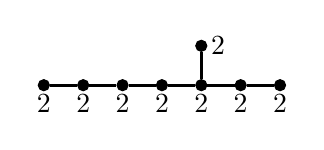
\begin{tikzpicture}
			\tikzset{dynode/.style={circle, draw, fill=black,
						minimum size=4pt, inner sep=0pt}}
			\tikzset{dyline/.style={line width=1pt}}
			\tikzset{dydash/.style={line width=1pt, dashed}}

			\begin{scope}[yshift=-10em, xshift=0]
				\node[dynode] (a1) at (0,0) {};
				\node[dynode] (a2) at (0.5,0) {};
				\node[dynode] (a3) at (1,0) {};
				\node[dynode] (a4) at (1.5,0) {};
				\node[dynode] (a5) at (2,0) {};
				\node[dynode] (a6) at (2.5,0) {};
				\node[dynode] (a7) at (3,0) {};
				\node[dynode] (a8) at (2,0.5) {};

				\draw[dyline] (a1) -- (a2) -- (a3) -- (a4) -- (a5) -- (a6) -- (a7);
				\draw[dyline] (a5) -- (a8);

				\node[below] () at (a1) {$2$};
				\node[below] () at (a2) {$2$};
				\node[below] () at (a3) {$2$};
				\node[below] () at (a4) {$2$};
				\node[below] () at (a5) {$2$};
				\node[below] () at (a6) {$2$};
				\node[below] () at (a7) {$2$};
				\node[right] () at (a8) {$2$};
			\end{scope}
		\end{tikzpicture}
		\quad\implies\quad
		\begin{pmatrix}
			2 & 1 &   &   &   &   &   &   \\
			1 & 2 & 1 &   &   &   &   &   \\
			  & 1 & 2 & 1 &   &   &   &   \\
			  &   & 1 & 2 & 1 &   &   &   \\
			  &   &   & 1 & 2 & 1 & 0 & 1 \\
			  &   &   &   & 1 & 2 & 1 & 0 \\
			  &   &   &   & 0 & 1 & 2 & 0 \\
			  &   &   &   & 1 & 0 & 0 & 2 \\
		\end{pmatrix}
	\]
	where each vertex of the tree is weighed by $2$.
\end{proposition}

It's interesting to note that if $Q$ is a matrix associated to a tree $T$, then $P(Q)$ has a $1$-skeleton homotopy equivalent to $T$. This connection between the $1$-skeleton and plumbing along a tree or graph was first noticed by Hirzebruch. It makes sense then why we'd care about matrices arising from trees instead of from general graphs which may contain cycles -- cycles break the simple-connectedness of the constructed manifold and are thereby much more complicated to work with.

% \begin{figure}[ht]\label{fig:negative-definite-trees}
% 	\centering
% 	\begin{tikzpicture}
% 		\tikzset{dynode/.style={circle, draw, fill=black,
% 					minimum size=4pt, inner sep=0pt}}
% 		\tikzset{dyline/.style={line width=1pt}}
% 		\tikzset{dydash/.style={line width=1pt, dashed}}
%
% 		\begin{scope}[yshift=0, xshift=22em]
% 			\node[dynode] (a1) at (0,0) {};
% 			\node[dynode] (a2) at (0.5,0) {};
% 			\node[dynode] (a3) at (1,0) {};
% 			\node[dynode] (a4) at (1.5,0) {};
% 			\node[dynode] (a5) at (2,0) {};
% 			\node[dynode] (a6) at (2.5,0) {};
% 			\node[dynode] (a7) at (3,0) {};
% 			\node[dynode] (a8) at (2,0.5) {};
%
% 			\draw[dyline] (a1) -- (a2) -- (a3) -- (a4) -- (a5) -- (a6) -- (a7);
% 			\draw[dyline] (a5) -- (a8);
%
% 			\node[] (l) at (1.75,-0.5) {$\E_8$};
% 		\end{scope}
%
% 		\begin{scope}[yshift=0, xshift=10em]
% 			\node[dynode] (a1) at (0,0) {};
% 			\node[dynode] (a2) at (0.5,0) {};
% 			\node[dynode] (a3) at (1,0) {};
% 			\node[dynode] (a4) at (1.5,0) {};
% 			\node[dynode] (a5) at (2,0) {};
% 			\node[dynode] (a6) at (2.5,0) {};
% 			\node[dynode] (a8) at (1.5,0.5) {};
%
% 			\draw[dyline] (a1) -- (a2) -- (a3) -- (a4) -- (a5) -- (a6);
% 			\draw[dyline] (a4) -- (a8);
%
% 			\node[] (l) at (1.5,-0.5) {$\E_7$};
% 		\end{scope}
%
% 		\begin{scope}[yshift=0, xshift=0]
% 			\node[dynode] (a1) at (0,0) {};
% 			\node[dynode] (a2) at (0.5,0) {};
% 			\node[dynode] (a3) at (1,0) {};
% 			\node[dynode] (a4) at (1.5,0) {};
% 			\node[dynode] (a5) at (2,0) {};
% 			\node[dynode] (a8) at (1,0.5) {};
%
% 			\draw[dyline] (a1) -- (a2) -- (a3) -- (a4) -- (a5);
% 			\draw[dyline] (a3) -- (a8);
%
% 			\node[] (l) at (1,-0.5) {$\E_6$};
% 		\end{scope}
%
% 		\begin{scope}[yshift=5em, xshift=3em]
% 			\node[dynode] (a1) at (0,0) {};
% 			\node[dynode] (a3) at (0.5,0) {};
% 			\node[dynode] (a4) at (1,0) {};
% 			\node[dynode] (a5) at (2.5,0) {};
% 			\node[dynode] (a6) at (3.0,0) {};
%
% 			\draw[dyline] (a1) -- (a3) -- (a4);
% 			\draw[dydash] (a4) -- (a5);
% 			\draw[dyline] (a5) -- (a6);
%
% 			\node[] (l) at (1.75,-0.5) {$\op{A}_n$};
% 		\end{scope}
%
% 		\begin{scope}[yshift=5em, xshift=17em]
% 			\node[dynode] (a1) at (0,0.4) {};
% 			\node[dynode] (a2) at (0,-0.4) {};
% 			\node[dynode] (a3) at (0.5,0) {};
% 			\node[dynode] (a4) at (1,0) {};
% 			\node[dynode] (a5) at (2.5,0) {};
% 			\node[dynode] (a6) at (3.0,0) {};
%
% 			\draw[dyline] (a1) -- (a3);
% 			\draw[dyline] (a2) -- (a3);
% 			\draw[dyline] (a3) -- (a4);
% 			\draw[dydash] (a4) -- (a5);
% 			\draw[dyline] (a5) -- (a6);
%
% 			\node[] (l) at (1.75,-0.5) {$\op{D}_n$};
% 		\end{scope}
% 	\end{tikzpicture}
% 	\vspace{1em}
% 	\caption{\todo{describe}}
% \end{figure}

\subsection{The Topology of Plumbed Manifolds}\label{sec:homotopy-type-plumbed}

In this section, we'll

\begin{proposition}
	If $\partial P^{2m}(Q)$ is a homotopy sphere then $Q$ is unimodular.
\end{proposition}

\begin{theorem}
	When $k>1$, $\partial P^{4k}(Q)$ is a homotopy sphere if and only if $Q$ is unimodular.
\end{theorem}


\begin{definition}
	The for $k>1$, the \defn{Milnor sphere} is the homotopy sphere $\partial P^{4k-1}(E_8)$.
\end{definition}

\subsection{Plumbing Constructions of 3-Manifolds}

Many of the results about the homotopy theory of plumbed manifolds in \cref{sec:homotopy-type-plumbed} only apply in dimensions $>4$. We can however still do the plumbing construction in $4$ dimensions, and it would be interesting to see what we get. In particular 

\todo{this section should be rewritten}

This $3$-manifold is known as (Poincar\'e) \defn{dodecahedral space} and has a beautiful geometric construction. We'll denote this space by $\mathscr{D}$. Aside from being a wonderful example of a non-Euclidean geometry, this space also was the first counter-example to an incorrect earlier form of the Poincar\'e hypothesised which stated that every homology $3$-sphere was also homeomorphic to the $3$-sphere. Much like exotic spheres are counter-examples to the smooth Poincar\'e hypothesis, in a similar vein the dodecahedral space can be thought of as a sort of ``proto exotic sphere'' serving as a counter-example to the ``proto Poincar\'e hypothesis''.

The classic construction of dodecahedral space $\mathscr{D}$ is due to Poincar\'e \todo{cite}. We begin by letting $\mathcal{D}\subset \R^3$ be a solid dodecahedron in three dimensional Euclidean space. The dodecahedron has 6 pairs of opposite pentagonal faces. Picking a clockwise spherical orientation on $\mathcal{D}$, we can glue together opposing faces with a minimal clockwise twist to line them up (see \cref{fig:dodecahedral_space_construction}). The resulting quotient space is a closed $3$-manifold, and this manifold is dodecahedral space $\mathscr{D}$.

\begin{figure}[ht]
	\centering
	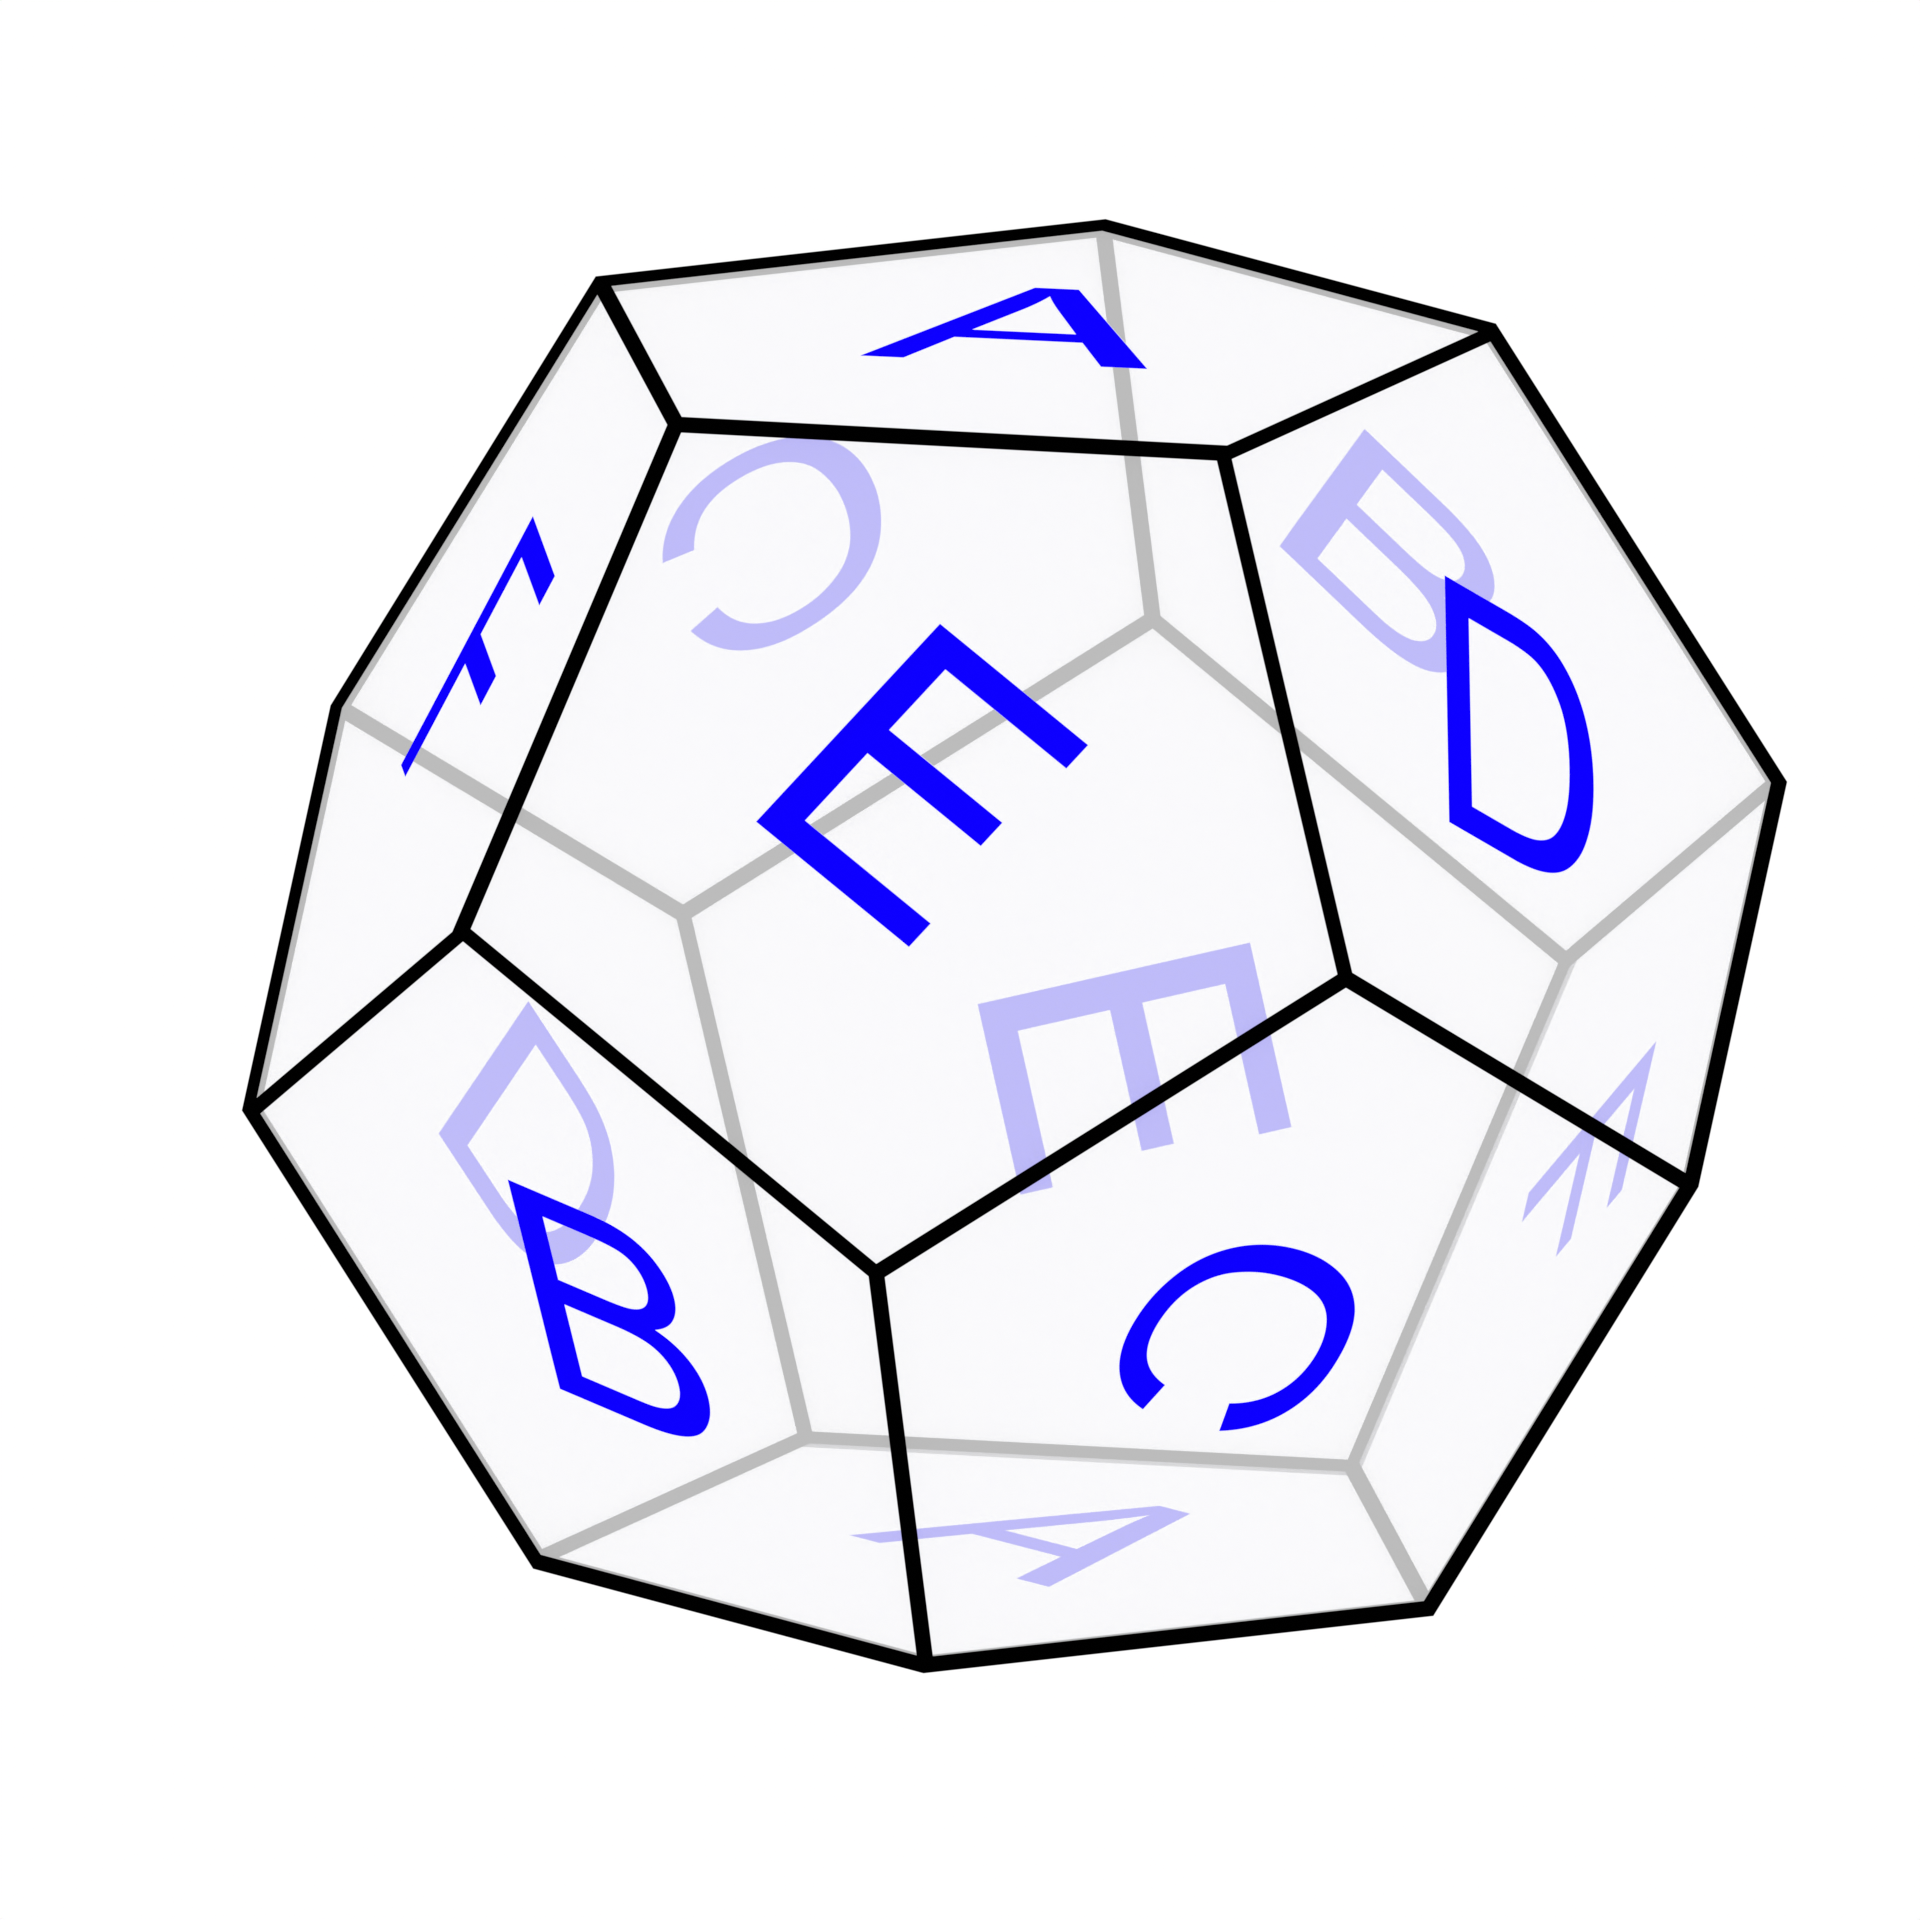
\includegraphics[width=2in]{graphics/temp-diagrams/dodecahedral-space-geometric-construction.png}
	\caption{Construction of Dodecahedral Space}\label{fig:dodecahedral_space_construction}
\end{figure}

Given this geometric construction, it should be fairly straightforward -- albeit tedious -- to compute the homology of dodecahedral space by means of a cellular decomposition. After such a computation, we would find that:
\begin{proposition}
	Dodecahedral space is a homology $3$-sphere.
\end{proposition}

While the first homology of dodecahedral space is trivial and incapable of differentiating dodecahedral space from a 3-sphere, the fundamental group reveals a much richer geometric structure. If we let $\SO_3$ act on $\R^3$ in the usual way, we can form the symmetry group $\Sym(\mathcal{D})\subset \SO_3$ of orientation preserving orthogonal transformations which leave the dodecahedron $\mathcal{D}$ unchanged. This is known as the \defn{icosahedral group}\footnote{The icosahedron and dodecahedron are dual, so the choice of icosahedral in the name is purely a historical convention.} $\mathrm{I}\subset \SO_3$, a group containing $60$ elements and isomorphic to the alternating group $A_5$. There is a double cover of $\SO_3$ by the $\Spin_3$ Lie group:
\[
	\SU_2\cong \Spin_3\lkxto[2:1] \SO_3
\]
The \defn{binary icosahedral group}, denoted $2\mathrm{I}$, is the preimage of $\mathrm{I}$ under this double cover and hence contains $120$ elements. Since there is an exceptional isomorphism $\SU_2\cong \Spin_3$, the binary icosahedral group admits a representation by unitary complex $2\times 2$ matrices.
We then have:
\begin{proposition}
	The fundamental group of dodecahedral space is the binary icosahedral group.
\end{proposition}
This hints at another interesting fact about the binary icosahedral group -- it is a \defn{perfect group}, which means that it's commutator subgroup is the entire group. By the Hurewicz isomorphism, it would follow that
\[
	\H_1(\mathscr{D}) \cong \Ab\left[ \pi_1(\mathscr{D})\right] \cong 2\mathrm{I}/[2\mathrm{I}, 2\mathrm{I}] = 0
\]
where $\Ab$ denotes the abelianization. This perfectness of the fundamental group thus ``hides'' the non-trivial topology of $\mathscr{D}$ from being detectable by homology. It's interesting to note that dodecahedral space and $S^3$ are the only homology $3$-spheres up to homeomorphism with finite fundamental groups.

There is also a useful construction of dodecahedral space which will later appear in our later study of Brieskorn manifolds in \todo{cite}. If we identify $\SU_2$ with the $3$-sphere of unit quaternions, we obtain the construction:

\begin{proposition}
	There is a diffeomorphism $\mathscr{D} \cong S^3 / 2\mathrm{I}$ expressing dodecahedral space as the quotient of the $3$-sphere under a proper group action by $2\mathrm{I}$.
\end{proposition}

Finally, let's see how the dodecahedral space and binary icosahedral group arises out of the plumbing construction we've worked with thus far.

\todo{write this section}

\begin{proposition}
	There is a diffeomorphism $\mathscr{D}\cong \partial P^4(\E_8)$.
\end{proposition}

\todo{citations}

\begin{remark}
	In the early 2000's, the Wilkinson Microwave Anisotropy Probe (WMAP) was launched to accurately map out the cosmic microwave background, i.e. leftover heat from the Big Bang. The observed lack of temperature correlations above 60$^\circ$ led astrophysicist Jean-Paul Luminet to propose a cosmological model \cite{luminet2003dodecahedral} where the shape of the universe is a dodecahedral space, explaining the lack of large scale correlations by means of the compact topology of space. In such a finite universe, larger temperature correlations simply wouldn't have enough room to form.
	While this model made some predictions aligning with observed cosmological data
	\cite{roukema2008dodecahedral}, higher resolution data by the later Planck spacecraft later seemed to suggest that the observable large scale topology is trivial, leading to the modern prevalence of the $\Lambda$CDM model as a standard model for cosmology.
\end{remark}

\section{Surgery Theory}

Now that we have the basic constructions out of the way, let's \todo{introduce}

\subsection{Groups of Homotopy Spheres}

\begin{definition}
	\todo{groups of homotopy spheres}
\end{definition}

\subsection{Fundamental Theorems of Surgery}

\begin{definition}
	\todo{surgical invariant $\sigma$}
\end{definition}

\begin{theorem}[Plumbing Theorem]\label{thm:plumbing-theorem}
	When $m>2$, there is a normal map \[(g,c) : (W,\partial W) \to (D^{2m}, S^{2m-1})\] which restricts to a homotopy equivalence $g|_{\partial W} : \partial W \to  S^{2m-1}$ with the invariant $\sigma(g,c)$ taking on any integer value.
\end{theorem}

% \section{Complex Singularities}
%
% Let $F\in \C[z_0,z_1\ldots, z_n]$ be a non-constant polynomial in $(n+1)$-complex variables.
% \begin{definition}
% 	The \defn{variety} of $F$ is the complex hypersurface given by the zero locus
% 	\[
% 		\V(F) = F^{-1}(0)=\left\{ z \in \C^{n+1}  F(z)=0\right\} \subset \C^{n+1}.
% 	\]
% \end{definition}
%
% \todo{cauchy riemann equations}
%
% \begin{definition}
% 	The \defn{gradient} of a complex analytic function $F : \C^{n+1} \to \C$ is the $(n+1)$-tuple
% 	\[
% 		\nabla_F = \left(\frac{\partial F}{\partial z_0}, \frac{\partial F}{\partial z_1},\ldots, \frac{\partial F}{\partial z_n}\right).
% 	\]
% 	\todo{better definition}
% \end{definition}
%
% \begin{definition}
% 	A point $w\in \V(F)$ is a (complex) \defn{singularity}[complex singularity] if $\nabla_F(w)$ vanishes. A singularity is \defn{isolated}[isolated singularity] if there is a neighborhood surrounding $w$ which contains no other singularities.
% \end{definition}
%
% \begin{theorem}
% 	For small $\varepsilon>0$ the intersection of $\V(F)$ with $D_\varepsilon(w)$
% \end{theorem}
%
% \begin{proposition}
% 	Every sufficiently small sphere around an isolated singularity of $F$ intersects $\V(F)$ transversally in a smooth manifold.
% \end{proposition}
%
% \begin{definition}
% 	Let $w\in \V(F)$ be an isolated singularity. The \defn{link} of $F$ at $w$ is the intersection
% 	\[
% 		\L(F, w) = \V(F) \cap S^{2n+1}_\varepsilon(w) = \left\{ z\in \C^{n+1}  F(z)=0\textrm{ and } |z-w|<\varepsilon\right\}
% 	\]
% 	where $\varepsilon > 0$ is some sufficiently small real number so that $\L(F,w)$ is a smooth manifold intersecting the sphere $S^{2n+1}_\varepsilon(w)$ transversally.
% \end{definition}
%
% When the isolated singularity is clear, we write $\L(F)$.
%
% \subsection{Brieskorn Manifolds}
% The simplest examples of complex polynomials with isolated singularities are \todo{this}
%
% \begin{definition}
% 	Let $(a_0,a_1,\ldots, a_n)$ be an $(n+1)$-tuple of integers greater than or equal to $2$. The \defn{Brieskorn polynomial} of the tuple $(a_0,a_1,\ldots, a_n)$ is given by
% 	\[
% 		F(z_0,z_1,\ldots, z_n) = z_0^{a_0} + z_1^{a_1} +\cdots + z_n^{a_n}.
% 	\]
% 	Correspondingly, we refer to $\V(F)$ as the \defn{Brieskorn variety} of the tuple and to the link at the origin $\L(F,0)$ origin as the \defn{Brieskorn manifold}. We'll use the notation
% 	\[
% 		\Sigma(a_0,a_1,\ldots, a_n) =\L(z_0^{a_0}+z_1^{a_1}+\cdots+z_n^{a_n}, 0)
% 	\]
% 	to refer to these Brieskorn manifolds.
% \end{definition}
%
%
% \begin{proposition}
% 	If $p,q\geq 2$, then $\Sigma(p,q)\subset S^3$ is the torus link of type $(p,q)$.
% \end{proposition}
%
% \begin{proposition}
% 	There is a homeomorphism $\Sigma(2,2,2)\cong \RP^3$.
% \end{proposition}
%
% \begin{proposition}
% 	There is a homeomorphism $\Sigma(2,3,5)\cong \mathscr{D}$.
% \end{proposition}
%
% \subsection{The Fibration Theorem}
%
% \begin{theorem}\label{thm:fibration}
% 	If $F$ is a complex polynomial in $(n+1)$-variables with an isolated singularity at the origin, then there is a smooth fiber bundle map
% 	\[
% 		\lkxfunc{\phi}{S^{2n+1}_\varepsilon - \L(F)}{S^1}{z}{\arg F(z).}
% 	\]
% \end{theorem}
%
% For a given angle $e^{i\theta}\in S^1$, we'll denote the fiber of the bundle $\phi$ as $F_\theta = \phi^{-1}(e^{i\theta})$.
%
% \begin{proposition}
% 	Each fiber $F_\theta$ is a smooth parallelizable $2n$-manifold.
% \end{proposition}
%
% \subsection{When is the link a topological sphere?}
%
% Let's fix a polynomial $F$ in $(n+1)$ complex variables
%
% \begin{proposition}
% 	If $n\neq 2$, then $\L$ is homeomorphic to the sphere $S^{2n-1}$ if and only if $\L$ has the homology of a sphere. In fact, $\L$ is a topological sphere if and only if the reduced homology $\widetilde{H}_{n-1}(\L)$ is trivial.
% \end{proposition}
%
% Let's now choose an orientation for $F_\theta$.
%
% \begin{proposition}
% 	The manifold $\L$ is a homology sphere if and only if the intersection form
% 	\[
% 		\lkxfunc{Q_{F_\theta}}{\H_n(F_\theta)\times \H_n(F_\theta)}{\Z}
% 	\]
% 	has determinant $\pm 1$ -- in other words if $Q_{F_\theta}$ is unimodular.
% \end{proposition}
%
% \section{Kervaire Invariant}
%
% \begin{theorem}[Brieskorn-Pham]
% \end{theorem}
%
% \begin{theorem}[Levine]
% 	If $n$ is odd, the Kervaire invariant is given by
% 	\[
% 		c(F_0) = \begin{cases}
% 			0 & \textrm{if }\Delta(-1)\equiv \pm 1\mod 8 \\
% 			1 & \textrm{if }\Delta(-1)\equiv \pm 3\mod 8
% 		\end{cases}
% 	\]
% \end{theorem}
%
% \begin{theorem}[Hirzebruch-Mayer] Smooth Brieskorn varieties are parallelizable.
% \end{theorem}
